\chapter{Fundamentals}
\label{chapter:fundamental}
In this first Chapter, we lay out the fundamentals used in the rest of this thesis. At the beginning, we will introduce basic definitions such as \emph{utterance}, \emph{sample} and \emph{conversation}. We will then follow up with an introduction into machine learning using a special variant of \emph{Neural Networks} (NN), called \emph{Recurrent Neural Network} (RNN). We show the basic principles behind it and explain problems this RNNs have in practice, and how the can be solved by utilizing other forms of RNNs. We then show how RNNs can be used to build models, called \emph{Sequence-To-Sequence} (seq2seq) models \cite{Sutskever:2014}, which are capable of learning and using a language in a conversational context.

The following introduction only covers a small part of the spectrum of possibilities with regard to the tasks these models can perform. We are restricting our explanations to the supervised learning use-case and ignore the unsupervised ones, even though they have a wide area of applications (e.g. dimensionality reduction, regression). A basic introduction into the principles of neural networks can be found in Appendix~\ref{fundamentals:neural_network}.\todo{label}

\section{Definitions}
\paragraph{Utterance} An \emph{utterance} is a single statement from one of the participants in a dialog. This means that an utterance can be either the initial statement or the response to this statement. An utterance may consist of several sentences, but they are always handled as if these sentences were uttered in one unbroken sequence by one participant without the second one interjecting.
\paragraph{Sample} A \emph{sample} is a combination of two utterances. The first is usually the utterance by the first participant, and the second on is the response to this first utterance by the second participant of the dialog.
\paragraph{Dialog} A \emph{dialog} is a conversation between two parties consisting of possibly multiple samples with two utterances each. An important distinction from how the term dialog is usually used in everyday life is, that we do not take the dialog context into account. This comes from the fact, that the model used in this thesis is not capable of handling context between multiple samples. We nevertheless us the term dialog to describe a string of multiple samples following each other.

The details on how dialogs are handled when training or doing inference with the model are described in detail in Chapter~\ref{methods}.

\section{Recurrent Neural Networks}
\emph{Recurrent neural networks} (RNN) are a special variation of the NNs described in Appendix~\ref{fundamentals:neural_network}. The main difference between them is, that RNNs have a recurrence built-in that allows them to adapt to problems which also have a temporal dimension and are dependent on data from different time steps to solve. We're also going into the problems such RNNs have due to their recurrence and how this problem can be solved by exploiting another form of RNN, called \emph{Long Short-Term Memory Networks} (LSTM).

\paragraph{Operating Principles of RNNs}
One of the main restrictions of vanilla NNs is the following: assume a task in which the NN is conditioned to output a prediction on tomorrow's weather given yesterday's. Now, if one would use a vanilla NN as described in Appendix~\ref{fundamentals:neural_network}, the main restriction would be that the NN has to make its prediction solely based on the weather information of the day before. Such a model does not take into account, that weather is not only dependent on the weather of the previous day, but also on the days before. This could be solved by feeding, say, the weather of the last week to the network instead of just the weather of the previous day. But if new scientific evidence now shows, that weather is not only dependent on last week, but also on the last month, probably the last year, we quickly get into problems due to the sheer size of a NN performing such tasks, because the input size grows rapidly. Also, such a NN would still be static in the sense that one cannot simply change the time-window used to feed to the network. If one settles for one month, it will always be able predict the weather based on the last month, but not any different time-window, otherwise the NN has to be retrained using another time-window in order to work again as before. RNNs (see Figure~\ref{fundamentals:rnn:internal_structure}) solve this problem by introducing a recurrence into the network, which allows it to exploit information not only from the current input, but also from inputs of the past. It does this by transferring a state, usually called the \emph{hidden state}, through the recurrence between different time steps. In a more compact way, one could say that this recurrence allows RNNs to ``exhibit dynamic behaviour across the temporal dimension of the input data''.

\begin{figure}[h]
	\label{fundamentals:rnn:internal_structure}
	\centering
	\includegraphics[width=10cm]{img/rnn_internal}
	\caption{Internal structure of a vanilla RNN cell.\protect\footnotemark}
\end{figure}


Before explaining how this recurrence can be used to solve the weather prediction problem, let's first show the equations used for the forward propagation in a RNN with a single cell. A single layer in an RNN is called a \emph{cell} and is basically a function which maps tuples of state and input to new tuples of a new state and an output $f\colon \mathbb{R}^n \times \mathbb{R}^m \rightarrow \mathbb{R}^n \times \mathbb{R}^m$, where $n$ signifies the size of the hidden state and $m$ the size of the output of the cell.\todo{For output and input $m$?}

The internal structure is similar to the one of NNs, except for the recurrence which we are going to elaborate on below.

\begin{equation}
\begin{split}
h_t & = \varphi_h(\mathbf{w}_h \cdot \mathbf{x}_t + \mathbf{u}_h \cdot \mathbf{h}_{t-1} + \mathbf{b}_h) \\
y_t & = \varphi_y(\mathbf{w}_y \cdot \mathbf{h}_t + \mathbf{b}_y)
\end{split}
\label{fundamentals:rnn:forward_equation:hidden}
\end{equation}
\todo{Format correctly!}

In the equations above, one can see different variables with different indices which we'll explain briefly:

\begin{itemize}[noitemsep]
	\item $x_t$ stands for the input at time step $t$.
	\item $y_t$ stands for the output of the network at time step $t$.
	\item $\mathbf{h}_t$ stands for the hidden state at time step $t$.
	\item $\mathbf{w}_h$, $\mathbf{w}_y$ and $\mathbf{u}_h$ are the weight matrices learned while training the model.
	\item $\mathbf{b}_h$ and $\mathbf{b}_y$ stand for the bias vectors used when computing the new hidden state or output respectively.
	\item $\varphi_y$ and $\varphi_h$ are the activation functions used to compute $y_t$ and $h_t$ respectively.
\end{itemize}

As seen above, at every time step $t$, the new hidden state $h_t$ and the output $y_t$ are computed. The value of $y_t$ can be seen as the prediction of the RNN at time step $t$ and the value of $h_t$ is the value that is passed to the same cell in the next time step $t+1$ for computing the next output $y_{t+1}$ (and hidden state $h_{t+1}$). As depicted in Figure \ref{fundamentals:rnn:internal_structure}, the hidden state $h_t$ is returned to the cell for computing the output $y_{t+1}$ and $h_{t+1}$. This is what an RNN allows to exhibit behaviour depending on data seen in past time steps: It can ``remember'' what it has already seen and store the information necessary for the prediction in the hidden state, which is passed along the temporal dimension when a RNN is run through multiple steps in time.
\footnotetext{http://r2rt.com/static/images/NH\_VanillaRNNcell.png}
To come back to our weather prediction problem, the recurrence and the hidden state passed along it allows the cell to remember what weather it has seen in the past and adjust its future predictions accordingly. The recurrence also solves the problem of time windows of different sizes: Since the recurrence allows the model to store the required informations in the hidden state at each time step and combine it with what it has already seen to make future predictions, it is not constrained to a fixed size of inputs required to make a prediction but instead uses all information it has already seen, no matter if the seen information is from the past five days or past five years, it can compress all this into the hidden state $h_t$.

While this is the solution for our problem of different window sizes, it is also a main bottleneck of the model: If one imagines, that the time window is past information is five years and we process these informations on a daily basis, we would need to remember the informations from around 1800 days. If we would now have 10 distinct features per day, this leads to 18'000 features to remember in total. Remembering means to compress the information into the hidden state, which is usually much smaller than 18'000 entries, reasonable values vary from 128 up to 4096 entries, depending on the structure and complexity of the problem. Another obstacle is, that the RNN cell has no way of forgetting information stored in the hidden state easily, as Equation \ref{fundamentals:rnn:forward_equation:hidden} only adds an addition to the hidden state $h_{t-1}$. Of course, in theory it is still possible that the RNN learns to forget insignificant information, but this is a really hard problem in practice, which is why we will introduce yet another form of RNN cell, called \emph{Long Short-Term Memory} cell that  not only solves this problem, but also partially the problem of unstable gradients explained in the next paragraph.

\paragraph{Vanishing / Exploding Gradients} The recurrent nature of RNNs can cause problems in practice, one of the most problematic is the vanishing gradients problem: While training such models, we condition the weight matrices $\mathbf{w}_h$, $\mathbf{w}_y$ and $\mathbf{u}$ via backpropagation by using gradient-descent in such a way, that the loss function is minimized with regard to these parameters for the given training samples. This means, that we have to compute the derivates of the loss function by using the chain-rule $dz/x = (dz/dy)(dy/dx)$. The entirety of all these derivates w.r.t. to the parameters is called the gradient. Since the gradient also flows through the activation functions $\varphi_h$ of the recurrence, this computations also include the derivates of this function. Most of the commonly used activation functions today have codomains in $\mathbb{R}$ and take on values in $[-1, +1]$ (e.g. $\operatorname{tanh}$). This means that multiplying many of this derivates possibly leads to vanishing values. This has a severe effect on training the RNN: If the values are vanishing, there is a point after which the network stops learning. This is because the change in weights becomes so small that the predictions will not change. This problem becomes especially acute when we use RNNs (or very deep NNs) with large window sizes as they act the same way as deep neural networks because they are unrolled when backpropagating.

Another problem which can occur is the opposite of the explained vanishing gradients: Exploding gradients. We talk about exploding gradients if the norm of the gradient becomes unreasonably large, to the point where it hurts the learning process severly. The gradient can explode due to the fact that the errors in the network propagate though an extended time window. This propagation takes the form of a multiplication of multiple Jacobbian matrices. If the norm of this matrices is larger than one, then the gradient might explode, especially if the used time window is large. A simple solution to this problem is to use gradient clipping~\cite{Pascanu:2013}. It solves the problem by clipping the norm value of the gradient if it exceeds a certain threshold.

The problem of vanishing gradients was first analyzed by Hochreiter in his diploma thesis \cite{Hochreiter:1991}. An analysis and in-depth explanation of the exploding gradient problem can be found in \cite{Pascanu:2012}. A more formal explanation of the problem, with links to dynamic systems and formal proofs, under which conditions these problems occur, can be found in \cite{Pascanu:2013}. The details on how backpropagation with gradient-descent is adapted to RNNs and time-dependent problems, called \emph{Truncated Backpropagation Through Time} or \emph{TBTT} in short, can be found in \cite{Werbos:1990}.

\paragraph{Long Short-Term Memory Networks} To solve the problem with vanishing gradients mentioned before, Schmidhuber and Hochreiter introduced an advanced version of a RNN cell, called \emph{Long Short-Term Memory}, or LSTM in short \cite{Hochreiter:1997}. The structure of this kind of cells is much more sophisticated then vanilla RNN cells, but it also solves the two most pressing problems: Vanishing gradients and the difficulty of forgetting stored information.

It does this by introducing the so-called \emph{gates} into the cell, which are nothing else than small NNs which are responsible for deciding which informations from the previous time step we are going to use from the old hidden state $h_{t-1}$, add to the new hidden state $h_t$ and use for the computation of the output $y_t$. There are three different gates in an LSTM cell (as depicted in Figure~\ref{fundamentals:lstm:internal_structure}):

\begin{itemize}
	\item \textbf{Input gate}: Is responsible to decide which part of the input is interesting and should be used to update the hidden state $h_{t-1}$ to become the new one $h_t$.
	\item \textbf{Forget gate}: Is responsible to decide which part of the hidden state $h_{t-1}$ the cell is going to forget.
	\item \textbf{Output gate}: Decides which part of the hidden state $h_t$ is used to compute the output $y_t$.
\end{itemize}

\begin{figure}[h]
	\centering
	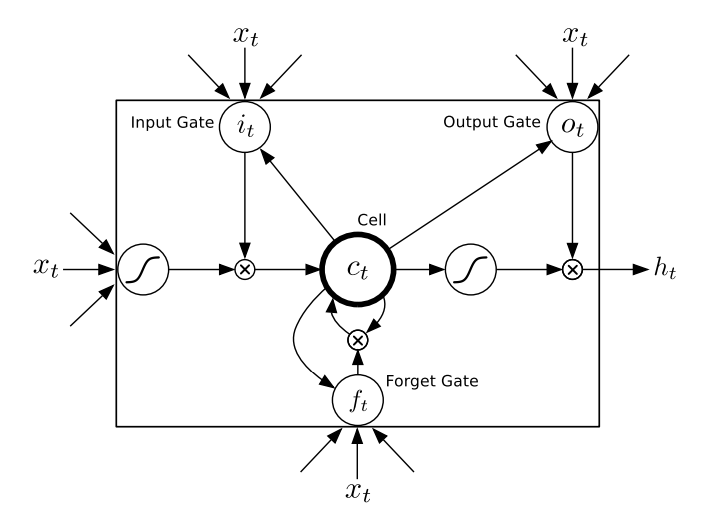
\includegraphics[width=10cm]{img/lstm_internal}
	\caption{Internal structure of a LSTM cell \cite{Graves:2013}.}
	\label{fundamentals:lstm:internal_structure}
\end{figure}

In theory, these gates do nothing more good than a plain RNN cell, as plain RNN cells are already Turing complete and hence can compute any desired function which is computable by a Turing machine \cite{Siegelmann:1995}. However, in practice this structure solves all of the aforementioned problems to at least some degree.

First, let us look into the vanishing gradient problem: The problem occured due to the fact, that the derivation of the activation function for the recurrence is used when calculating the updates of the weight parameters by performing backpropagation with gradient-descent. This can lead to vanishing (if the derivate is below 1) or exploding (if the derivate is above 1) gradients. The LSTM cell solves this problem by not applying an activation function on the recurrence, but rather using the identity function $f(x) = x$ whose derivation is always $1$. This practically solves this problem because the gradients do not vanish anymore.

The second problem is that an RNN cell has no explicit way of forgetting information stored in the hidden state. This is solved by the introduction of gates which allow the cell to decide at each time step $t$, which information to keep, forget and store based on the last hidden state $h_{t-1}$ and the current input $x_t$. With this structures in place, the LSTM cell is able to track long-term dependencies much better than a vanilla RNN cell.

There are more details regarding the LSTM cell, like the forget bias and peephole connections, which can be looked up in a empirical study by Greff et al. \cite{Greff:2016}. There are even more architectures for RNN cells like Gated Recurrent Unit \cite{Chung:2014} and Convolutional LSTM \cite{Xingjian:2015}, which we will not describe in detail in this thesis.

\section{Sequence-To-Sequence Learning}
\label{fundamentals:seq2seq}
The RNN and LSTM cells described in the preceeding Chapter can now be used to build so-called \emph{Sequence-To-Sequence} (seq2seq) models. They were first introduced by several people around the same time \cite{Sutskever:2014}\cite{Kalchbrenner:2013}\cite{Cho:2014}, mainly for usage in the context of machine translation tasks, but they can also serve as a generic model for learning to map arbitrary input to output sequences. They have shown, that such models can be successfully adapted to machine translation tasks and exhibit almost state-of-the-art performance. For more general information on where and how seq2seq models used we refer to Chapter \ref{related_work}. In the following paragraphs, we are going to explain the basic idea behind the model and how each of its parts, called encoder and decoder, work when applied to conversational modeling.

\paragraph{Model}
The basic idea behind the model is to separate the parts necessary to understand and parse the input sequence, called the \emph{encoder}, from the part that is responsible for generating the output sequence, called the \emph{decoder} (see Figure \ref{fundamentals:seq2seq:internal_structure}). Both the encoder and decoder can be any kind of RNN cell, be it GRU, LSTM or any other. The encoder is fed with the input sequence through multiple time steps, as an example one could say that for example each word of an input sentence is fed to the encoder one at a time. Through this process, the encoder starts to build its internal hidden state, updates it every time a new word is fed and passes it along the recurrence to serve as the initial state of the cell at the next time step. After the input sequence is fully processed by the encoder, it then passes the information collected in the hidden state, in the context of seq2seq models also called \emph{thought vector}, to the decoder cell. The decoder cell then uses this hidden state as its own, internal, initial state and starts to produce the output sequence, one token per time step, after its fed with a dedicated \texttt{GO} token (also depicted in Figure~\ref{fundamentals:seq2seq:internal_structure}). The tokens are produced by feeding the final state of the decoder cell to a softmax classification layer which outputs a probability distribution over the words in the vocabulary. It then usually chooses the ``best'' token to output in a greedy fashion by simply selecting the token with the highest probability after the softmax layer has been applied. The details on how the decoding exactly works are described in the paragraph \emph{Decoding Approaches} below. In general, the decoder tries to construct a sensible output at every time step, in our case this corresponds to the current input word, $t$ given the hidden state from the decoder at time step $t-1$ and the last output $y_{t-1}$.

\begin{figure}[h]
	\centering
	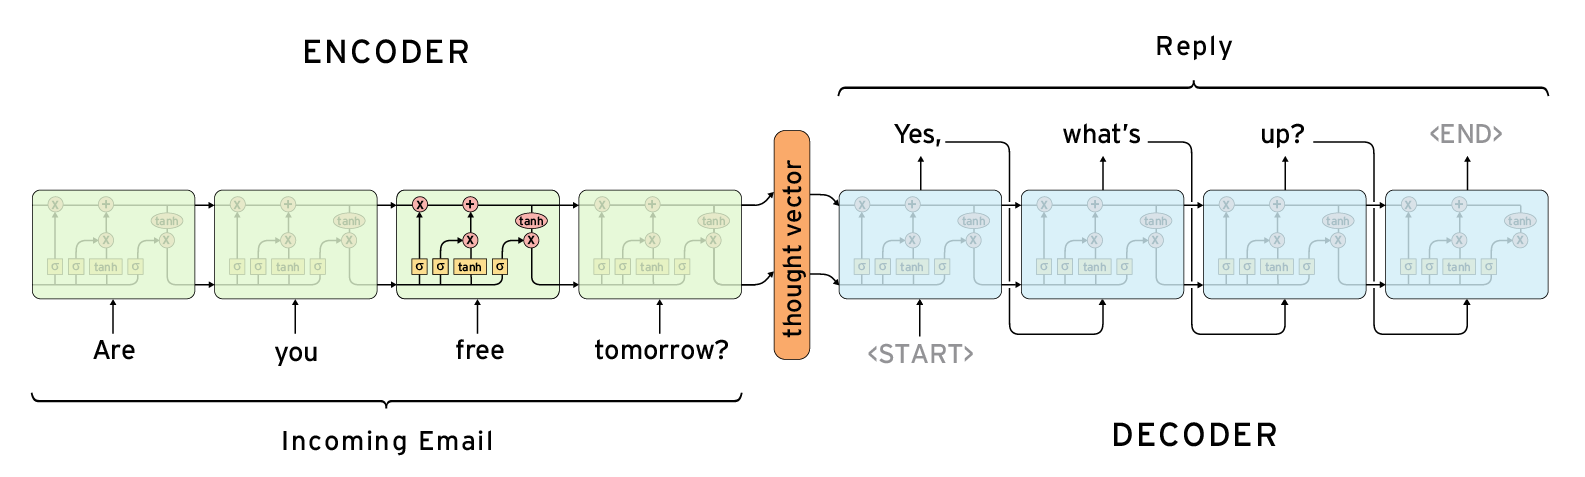
\includegraphics[width=14cm]{img/seq2seq_internal}
	\caption{Internal structure of a Sequence-To-Sequence Model.\protect\footnotemark}
	\label{fundamentals:seq2seq:internal_structure}
\end{figure}
\footnotetext{http://suriyadeepan.github.io/2016-12-31-practical-seq2seq/}

Such a model is also called an \emph{end-to-end} model because it, being fully differentiable, can be trained by using backpropagation with gradient-descent with ease. The training works by having pairs of input-output samples which are then used to train the network and condition it to generate the expected output given the input sequence. This is done by feeding the network the expected words as inputs at each time step which allows for gradient-descent to be applied. Formally, if we're talking about language modeling, the model is conditioned to optimize the conditional probability $p(y_1, \dots, y_{T}|x_1, \dots, x_{T'})$, where $T$ is the length of the input sequence and $T'$ the length of the corresponding output sequence. As said before, the encoder cell produces a thought vector $v$, which is nothing more than its hidden state after it has processed the input sequence $x_1, \dots, x_2$, and passes this to the decoder for generating the output sequence. The decoder is then trained to compute the probability of $y_1, \dots, y_T$ given the thought vector $v$:

\begin{equation}
p(y_1,\dots,y_{T'}|x_1,\dots,x_{T}) = \prod_{t=1}^{T'} p(y_t|v,y_1,\dots,y_{t-1})
\end{equation}
\todo{Describe more?}

Each of the terms $p(y_t|v,y_1,\dots,y_{t-1})$ in the product represents a distribution over all words of the vocabulary that is computed when applying the softmax layer at the end. What might be perplexing to the reader is that on the right hand side of the equation, the inputs $x_1,x_2,\dots,x_T$ are left out. This has to do with the fact that the decoder produces its prediction solely based on the thought vector $v$ produced by the encoder and the decoders previous predictions $y_1,\dots,y_{t-1}$ (in a formulation without soft-attention, see below).

If we look at the example depicted in Figure \ref{fundamentals:seq2seq:internal_structure}, the generation of the output sequence is done as follows:

\begin{enumerate}[noitemsep]
	\item Feed the encoder the current input word $x_t$ and update its hidden state accordingly. The output of the cell can be ignored.
	\item Repeat step 1 until the inputs $x_1,\dots,x_{T}$ are exhausted.
	\item Pass the hidden state of the encoder cell to the decoder cell after the first has processed the last word $x_T$ of the input sequence.
	\item Initialize the decoder with the given hidden state and feed it the dedicated \texttt{GO} token.
	\item Store the output token $y_t$ of the decoder cell. After this, it depends on which decoding approach is used to generate the output sequence:
	\begin{enumerate}
		\item In case of a greedy decoder, simply feed the output $y_t$ and hidden state $h_t$ back in to the decoder cell to produce the next output token $y_{t+1}$ and hidden state $h_{t+1}$.
		\item In case of a beam-search decoder, select the $N$ outputs $y_1,\dots,y_{N}$ with the highest probability and store them together with the respective hidden states. Feed each of this outputs with the respective hidden state back into the decoder cell.
	\end{enumerate}
	\item Repeat step 5 until the decoder either outputs an \texttt{EOS} token or the maximum length $T'$ for the output is reached.
\end{enumerate}

The concatenated outputs $y_1,...,y_{T'}$ are the output of the model. The exact decoding approaches are described in more detail in the \emph{Decoding Approaches} paragraph below. Generally speaking, such models can be used for \emph{any} sequence-to-sequence problem, not just language modeling, as long as it is possible to define a probability distribution over the output tokens $y_t$. Another fact worth mentioning is, that we described this model when using a single RNN cell for encoding and decoding, but it is indeed possible to use multiple cells for each of these parts.

\paragraph{Soft-Attention Mechanism}
\label{fundamentals:soft_attention}
\todo{revisit one more time!}
Imagine you have been asked to solve the following simple task: Read a longer text about a certain topic. At the end of the text, there are several questions regarding this text and you have to answer them. How does a human approach such a task? At least a part of the people start by reading the text through one time and then start to answer the questions. A normal human cannot remember the whole content of the text (since it is a long one), so what it does is to focus on a single question and try to find the answer by revisiting the text. This essentially means that the participant in this task \emph{focuses} their \emph{attention} on single parts of the text instead of the text as a whole. This is basically what the \emph{soft-attention} \cite{Bahdanau:2014} mechanism is all about. Let us adapt the introductory example on how this behavior could be adapted to seq2seq models and how it helps to solve tasks.

As mentioned before, the main bottleneck of seq2seq models is that the encoder has to compress all the information it has processed into its thought vector. The thought vector is then passed to the decoder which tries to come up with a meaningful answer to the information stored in the thought vector. If a long text is compressed into the thought vector, this might not be an easy task to solve as the information has to be compressed too much. The attention mechanism helps by solving this issue by allowing the decoder to look at all thought vectors of the encoder at all time steps via a weighted sum. 

We are going to describe the attention mechanism in more detail now and follow the explanations in \cite{Vinyals:2015:Foreign} to do so. Formally, the attention mechanism works as follows: Consider that we already have all hidden states of the encoder $\mathbf{H} = \{h_1,\dots,h_t\}$ at the time we start decoding, where $t$ stands for the last time step the encoder had to process an input word. We also have the hidden states of the decoder $\mathbf{D} = \{d_1,\dots,d_t\}$ (since attention is applied after the cell has predicted the current token at time step $t$). We use the same number of hidden states in $\mathbf{H}$ and $\mathbf{D}$ for the sake of simplicity, but it could be possible that there are a different number of time steps for the encoder and decoder. The attention vector $d_t$ is computed with the following equations:

\begin{equation}
\label{fundamentals:attention:equations}
\begin{split}
	u^t_i & = v^T \tanh(W_1 h_i + W_2 d_t) \\
	a^t_i & = \operatorname{softmax}(u^t_i) \\
	d'_t & = \sum_{i=1}^{t} a^t_i h_i
\end{split}
\end{equation}

The index $t$ stands for the current time step as almost anywhere else. The index $i$ ranges from $1$ to the number of steps we have computed in the encoder, which is equal to $t$ in our case. The vector $v$ and the matrices $W_1$ and $W_2$ contain the learnable parameters for the attention mechanism. The vector $u^t$ is of length $t$ and its entries signify, how much attention should be put on the hidden state $h_i$ of the encoder. By applying a softmax layer on the vector $u^t$, we turn it into the probability distribution $a^t$ over all hidden states $\mathbf{H}$ from the encoder. The final computation of the $d'_t$ is then done by computing the weighted sum between the weight vector $a^t$ and the respective hidden state $h_i$ from the encoder. This vector $d'_t$, also called context vector, is then concatenated together with the current hidden state of the decoder $d_t$ to become the new hidden state with which we go on predicting the next output token at time step $t+1$.

The weights $W_1$ and $W_2$, as well as the values in the vector $v$, are learned while training the model. This means, that ability to be ``attentive'' is something the model has to learn and hence cannot be added after the training. This also means that choice on what the model attends is not only dependent on the current sample, but also on the task in general.

\begin{figure}[H]
	\centering
	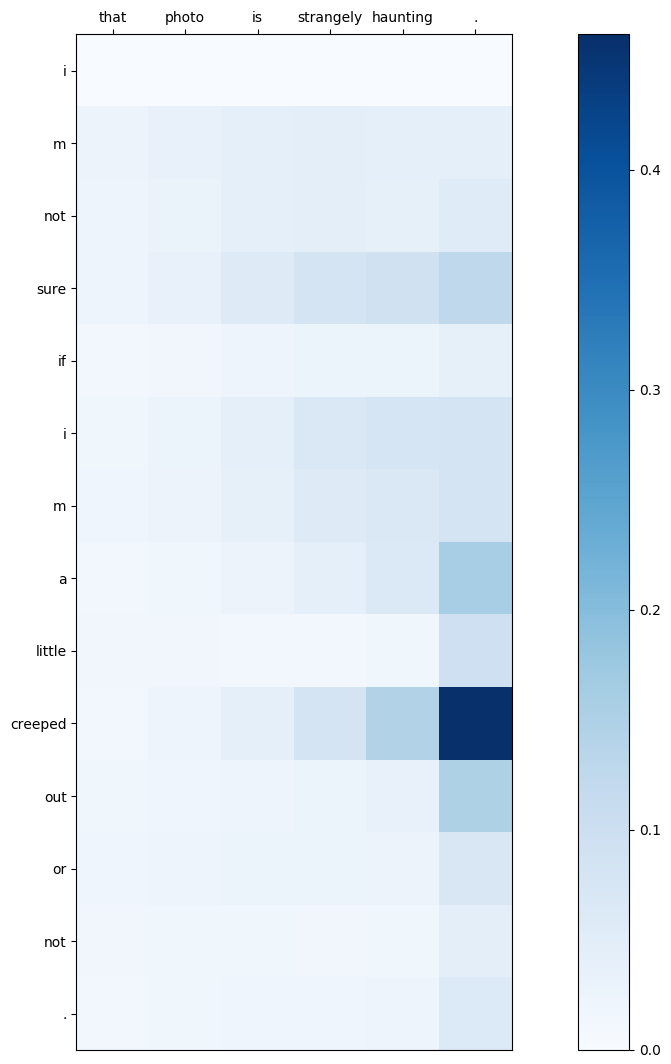
\includegraphics[width=10cm]{img/attention_heatmap_example}
	\caption{Example on how attention can be visualized using a heatmap. The input sequence is on the x-axis and the respective response on the y-axis. Each line in the heatmap can be interpreted as the probability distribution over the thought vectors of the encoder which the decoder accesses at each decoding step.}
	\label{fundamentals:seq2seq:attention_weights_visualization}
\end{figure}\todo{Erklären, dass dieses Beispiel eine eher sinnlose attention aufweist?}

The name \emph{soft}-attention comes from the fact, that this kind of attention mechanism is fully differentiable and hence can be simply plugged into any existing NN architecture. The other kind of of attention is the so-called \emph{hard}-attention mechanism which in contrast samples a random thought vector of the encoder and because of that, it is not fully differentiable and hence cannot simply be added to an existing system that uses back-propagation and gradient-descent without modifications.

We have only explained on how soft-attention can be used in a context where we process language. However, the attention mechanism itself originated from the computer vision area \cite{Desimone:1995}\cite{Itti:1998}\cite{Mnih:2014} and has a wide range of applications there \cite{Gregor:2015}\cite{Xu:2015}\cite{Cho:2015}. The mechanism can be adapted to any kind of problem and model, not just computer vision or NLP, as long as the model has any way of accessing the input data.

\paragraph{Decoding Approaches}
\label{fundamentals:decoding_approaches}
In the following paragraph, we are going to elaborate on two decoding approaches that we are going to use in our experiments: \emph{greedy} decoding and \emph{beam-search} decoding.

Greedy decoding is the simpler of the two variants. When using it, the output $y_t$ of the model using it is simply the token with the highest probability after the softmax layer has been applied on the last hidden state $h_t$ of the decoder at time $t$. It then goes on by feeding in the hidden state $h_t$ and the last output word $y_t$ to produce the output token $y_{t+1}$ for the next time step $t+1$. This variant is really simple to implement, but also has its flaws: Since the decoder is working in a local and greedy fashion, it does not know beforehand what kind of sentence it would predict best, and hence has to stick with local optima on each time step $t$ by returning the word with the highest probability after applying the softmax.

Beam-search tries to fix or at least minimize this problem by not only considering a single candidate sequence but instead focuses on the $m$ different sequences that are most promising. The variable $m$ is called the \emph{beam width} and signifies how much possible candidate sequences are under consideration. The approach itself works by doing the usual computation and process the input sequence with the encoder cell at the beginning. The last hidden state of this encoder is then passed to the decoder which starts to do the beam search. It begins by using the last hidden state (and the \texttt{GO} token) to predict the first word of the output in the same way as the greedy decoder does. But now, instead of simply choosing the next token to be the one with the highest probability, the decoder stores the $m$ tokens with the highest probability. In the next step, the decoder is now fed with all of the $m$ tokens produced in the step before and their respective hidden states. After this seconds step, the decoder has to \emph{prune} the beams by deciding which of the $m$ sequences it wants to keep and which it wants to discard. This has to be done, because after the second step, there are actually $m^2$ candidate sequences combined in all beams, which violates the rule that there may be atmost $m$ beams. The $m^2$ candidate sequences are ranked by the sum of the log-probabilities of all the predicted words at each time step in every beam. Instead of using the plain probabilities from the softmax layer, the log-probabilites are used to ensure that the computation is numerically stable, as the multiplication of a lot of small values can lead to instabilities. After the ranking, the  This process is then carried out until we reach an \texttt{EOS} token in one the beams or the maximum number of allowed time steps in the decoder is reached. To decide, which is the best predicted sequence at the end of the beam-search, we again look at the sum of the log-probabilites and take the one with the value which is nearest to $0$ (as a sum of log-probabilities is a sum of negative numbers).

\begin{figure}[H]
	\label{fundamentals:seq2seq:beam_search}
	\centering
	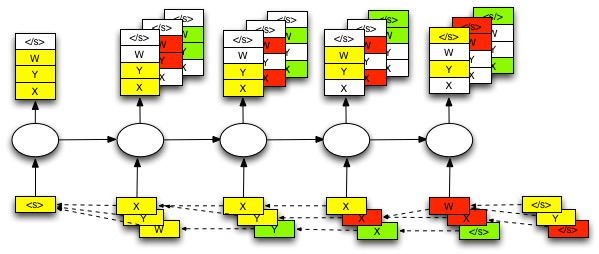
\includegraphics[width=12cm]{img/beam_search_visualization}
	\caption{Visualization on how beam search works in the context of seq2seq models.\protect\footnotemark}
\end{figure}
\footnotetext{https://github.com/tensorflow/tensorflow/issues/654}

\section{Performance Metrics}
\label{fundamentals:metrics}
In this Section, we are going to introduce the main performance metrics used in this thesis to asses the performance of the trained models.

\paragraph{Cross-Entropy Loss} For our model, we are using the \emph{Cross-Entropy} loss function while training. It can be used to measure how well an expected probability distribution $p$ is predicted by a trained model, where the predicted distribution is denoted as $q$. In our case, the probability distribution $p(x)$ is the distribution of the words predicted by the decoder at the time step $t$ and $q(x)$ is the expected distribution for the given sample $x$. The loss function is defined via the following equation where $X$ stands for the whole training dataset:

\begin{equation}
H(p, q) = -\sum_{x \in X} p(x) \log_2 q(x)
\end{equation}
\todo{Check one more time!}

In the case of sequence-to-sequence learning, the expected probability is a one-hot encoded vector with a $1$ at the entry of the expected word at time step $t$ and $0$ everywhere else. This loss function can be used for training a seq2seq model (or any model which predicts probability distributions in a broader sense) and it can then also be used to calculate the perplexity of the model, which we are going to elaborate on below.

\paragraph{Perplexity} The perplexity is another metric for measuring how good a language model will predict the sentences in the test dataset and is closely tied to the cross-entropy loss function. The value of the perplexity can be computed by raising the value of the cross-entropy loss function to the power of $2$. The perplexity can be computed by the following equation:

\begin{equation}
\operatorname{perplexity}(X) = 2^{H(X)}
\end{equation}

The perplexity tells ``how good'' a language model is. More formally, it tells us how good the model reproduces the samples seen in the test set. For example, a ``dumb'' model would predict each word with equal probability, which would be $1/|V|$, where $|V|$ is the vocabulary size. This does not reflect reality, as certain words are much more likely to occur often in language.

\paragraph{Sent2Vec Similarity}\label{fundamentals:sent2vec_test} We were seeking for a third performance metric, since the perplexity is simply $2$ raised to the power $H(X)$. This means, we effectively have one performance metric to use. To fix this problem, we also investigated into using Sent2Vec\footnote{https://github.com/epfml/sent2vec} \cite{Pgj:2017} for measuring the semantic difference of the sentences generated by the model when testing it after it has been trained. We propose the following way to test the model:

\begin{enumerate}[noitemsep]
	\item Allocate a variable for storing the sum of similarities.
	\item Repeat the following steps until all samples in the test set are exhausted:
	\begin{enumerate}[noitemsep]
		\item Create prediction for the given input sentence.
		\item Embed the generated and expected sentences via \texttt{Sent2Vec} to obtain n-dimensional embedding vectors for both of them.
		\item Measure the distance by using the cosine similarity between the embeddings in the n-dimensional vector space.
		\item Add this similarity to the sum of similarities.
	\end{enumerate}
	\item Divide the sum of all collected similarities by the number of samples. This is the final result which can be used as a metric.
\end{enumerate}

This procedure allows us to further analyze the performance of the model by comparing the semantic similarities between the expected and the generated answers in the $n$-dimensional vector space, where $n$ is the dimensionality of the sentence embeddings. For example, when the expected output sentence is ``I feel good, how about you?'' and the answer generated by the model is ``I'm fine, you?'', the similarity measurement should return a value close to $1$ since we would expect that this sentences are embedded closely to each other due to the semantic similarity of the content. In contrast, when the output of the model is ``I really love cupcakes'' and the expected sentence is still the same, the similarity measure should become close to $0$ to signify that there is a large mismatch between the meaning of the expected and generated sentence.

